\documentclass{article}
\usepackage[margin=1in]{geometry}
\usepackage{longtable}
\usepackage{enumitem}
\usepackage{listings}
\usepackage{xcolor}
\usepackage{hyperref}
\usepackage{graphicx}
\usepackage{adjustbox}
\usepackage{float}
\lstdefinelanguage{json}{
  basicstyle=\ttfamily\small,
  numbers=left,
  numberstyle=\tiny\color{gray},
  stepnumber=1,
  numbersep=5pt,
  showstringspaces=false,
  breaklines=true,
  frame=single,
  backgroundcolor=\color{gray!10},
  literate=
   *{0}{{{\color{blue}0}}}{1}
    {1}{{{\color{blue}1}}}{1}
    {2}{{{\color{blue}2}}}{1}
    {3}{{{\color{blue}3}}}{1}
    {4}{{{\color{blue}4}}}{1}
    {5}{{{\color{blue}5}}}{1}
    {6}{{{\color{blue}6}}}{1}
    {7}{{{\color{blue}7}}}{1}
    {8}{{{\color{blue}8}}}{1}
    {9}{{{\color{blue}9}}}{1}
    {:}{{{\color{black}:}}}{1}
    {,}{{{\color{black},}}}{1}
    {"}{{{\color{teal}"}}}{1}
}

\title{Biomass Chain of Custody (CoC) Data Standard}
\date{}
\begin{document}
\maketitle

\section{Overview / Purpose}
This document defines a flexible, open-access data standard for tracking biomass through a certified, auditable chain of custody (CoC) system. It is designed to support compliance with California state laws (SB 498, SB 1383), ensure regulatory transparency, and streamline reporting burdens for biomass supply chain actors.

\textbf{Goals:}
\begin{itemize}[noitemsep]
    \item Enable secure, low-cost, and scalable biomass tracking
    \item Support multiple regulatory reporting pathways
    \item Promote interoperability between public and private systems
    \item Promote interoperability between various biomass sustainability standards
    \item Provide data structure guidance for software developers, facilities, and government agencies
\end{itemize}

\section{Scope}
\subsection*{Covered Materials}
Biomass categories defined under this standard, aligned with international and certification scheme taxonomies, include:
\begin{itemize}[noitemsep]
    \item \textbf{Category 1:} Woody biomass from Forest Management Units (FMU)
    \item \textbf{Category 2:} Woody biomass from small Forest Management Units (FMU less than 500 hectares)
    \item \textbf{Category 3:} Residues from nature and landscape management (e.g., urban green space cuttings)
    \item \textbf{Category 4:} Agricultural residues (e.g., straw, stalks)
    \item \textbf{Category 5:} Biogenic residues and waste flows (secondary and tertiary residual streams)
    \item \textbf{Category 6:} Marine biomass 
\end{itemize}

\subsection*{Biomass Types}
The standard distinguishes two overarching biomass types for certification and subsidy eligibility:
\begin{itemize}[noitemsep]
    \item \textbf{Sustainable biomass:} Biomass that meets all applicable sustainability criteria selected state and international regulations or sustainability standards. 
    \item \textbf{Controlled biomass:} Category 1 or 2 biomass that meets a defined subset of criteria (e.g., risk assessment, forest management requirements) but not the full set; limited to 30\% of subsidy-eligible volumes.
\end{itemize}

\subsection*{Participating Entities}
\begin{itemize}[noitemsep]
    \item Harvesters / Collectors
    \item Transfer Stations / Processors
    \item Biomass Conversion Facilities
    \item Composters, Biochar Producers, Bioenergy Facilities
    \item Regulators (CalRecycle, CARB, LEA)
\end{itemize}

\subsection*{Supported CoC Models}
\begin{itemize}[noitemsep]
    \item Mass Balance
    \item Physical Separation
    \item Crediting
\end{itemize}

\subsection*{Interoperable Systems}
\begin{itemize}[noitemsep]
    \item CalRecycle
    \item CalTrace
    \item FSC Trace
\end{itemize}

\section{Event \& Reporting Framework}
\begin{longtable}{|p{4cm}|p{4cm}|p{4cm}|p{4cm}|}
\hline
\textbf{Event} & \textbf{Trigger} & \textbf{Reported To} & \textbf{Required Fields} \\
\hline
Material Created & Material batch generated & CoC System & material\_id, origin, attributes \\
Material Transferred & Shipment leaves sender & CoC System, CalRecycle & transaction\_id, documentation, receiver\_id \\
Certificate Issued & Facility certifies batch & CoC System & claim\_id, material\_id, scheme \\
Report Submitted & SB 498/SB 1383 due date & CalRecycle, CARB & Facility roll-up of totals, recovery \\
\hline
\end{longtable}

\section{System Integration Guidelines}
\subsection*{Interfaces}
\begin{itemize}[noitemsep]
    \item CalRecycle RDDS: batch data upload + quarterly summaries
    \item CARB LCFS: load-level + mass balance compliance
    \item SBP DTS: optional plug-in for certified exporters
\end{itemize}

\subsection*{Formats}
\begin{itemize}[noitemsep]
    \item JSON (preferred)
    \item CSV (fallback)
    \item XML (fallback, optional)
    \item RESTful API / Secure upload
\end{itemize}

\section{Governance \& Versioning}
\begin{itemize}[noitemsep]
    \item \textbf{Maintainer:} Carbon Direct (initial release)
    \item \textbf{Versioning:} Semantic (e.g., 1.0.0)
    \item \textbf{Update Cycle:} Semiannual review + stakeholder input
    \item \textbf{Change Proposals:} Via GitHub issues or agency feedback portal
\end{itemize}

\section{Appendices}
\subsection*{A. Glossary}
\begin{itemize}[noitemsep]
    \item \textbf{BDT:} Bone Dry Ton
    \item \textbf{CoC:} Chain of Custody
    \item \textbf{RDDS:} Recycling and Disposal Reporting System
\end{itemize}

\subsection*{B. Code Lists}
\begin{itemize}[noitemsep]
    \item Material Types: wood\_waste, ag\_residues, pulp, sawmill\_residues
    \item Entity Types: harvester, processor, end\_user, etc. 
    \item Certification Schemes: FSC, SBP, SFI, LCFS
\end{itemize}

\subsection*{C. Example JSON Payloads}
\begin{lstlisting}[language=json]
{
  "transaction": {
    "id": "TX-2025-00123",
    "timestamp": "2025-05-01T00:00:00Z",
    "material_id": "BATCH-1001",
    "sender_id": "ORG-001",
    "receiver_id": "ORG-009"
  },
  "organizations": [
    {
      "id": "ORG-001",
      "name": "Green Biomass Ltd.",
      "type": "harvester"
    },
    {
      "id": "ORG-009",
      "name": "Urban Heat & Power Co.",
      "type": "end_user"
    }
  ],
  "material": {
    "id": "BATCH-1001",
    "category": "sawmill_residues",
    "certification": "FSC",
    "quantity": 50.0,
    "moisture_content": 8.5,
    "certificate_id": "CERT-001",
    "emissions_profile_id": "EMISS-001"
  },
  "certificate": {
    "id": "FSC-COC-100",
    "scheme": "FSC",
    "status": "active",
    "issue_date": "2024-06-01",
    "expiry_date": "2029-06-01"
  },
  "emissions_profile": {
    "id": "EMISS-001",
    "transport_distance": 350.0,
    "ghg_emissions": {
      "fossil_fuel_comparator": "91 gCO2e/MJ",
      "fuel_used_liters": 60.0
    }
  }
}
\end{lstlisting}

\subsection*{D. Abstracted Entity Relationship Diagram for CoC}

\begin{figure}[H]
  \centering
  \adjustbox{max width=\textwidth, max height=0.8\textheight}{
    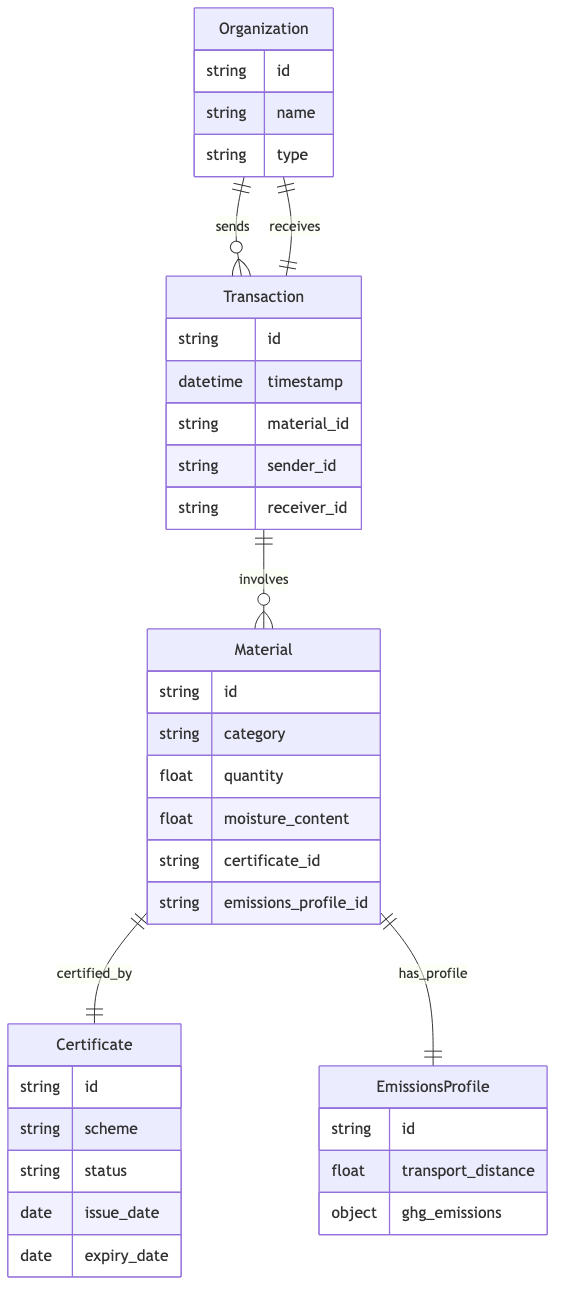
\includegraphics{updated_coc_erd_with_roles.png}
  }
  \caption{Abstracted CoC ERD}
  \label{fig:updated_coc_erd}
\end{figure}
\subsection*{E. SB 498 \& SB 1383 Data Crosswalk}

This section maps key data elements in the Chain of Custody (CoC) data standard to the specific reporting requirements of California Senate Bills 498 and 1383. The goal is to ensure compliance with regulatory mandates while minimizing duplicative data entry for reporting entities.

\subsubsection*{E.1 Overview of SB 498}

SB 498 requires biomass conversion facilities to submit annual reports to CalRecycle detailing the types and quantities of biomass materials processed, their sources, and the conversion technologies employed. The reporting focuses on:

\begin{itemize}[noitemsep]
    \item Categorization of biomass materials (e.g., agricultural residues, urban wood waste)
    \item Quantities processed and converted (units) - may need to be obscured to some users in the CoC as competitive or proprietary.
    \item Source sectors (e.g., agriculture, forestry, urban)
    \item Conversion technologies used (e.g., combustion, gasification)
    \item Facility-level operational data
\end{itemize}

\textbf{Reporting Deadline:} April 1st annually for the preceding calendar year.

\subsubsection*{E.2 Overview of SB 1383}

SB 1383 mandates the reduction of organic waste disposal in landfills to cut methane emissions. Jurisdictions and relevant entities are required to:

\begin{itemize}[noitemsep]
    \item Provide organic waste collection services to all residents and businesses
    \item Monitor and minimize contamination in organic waste streams
    \item Procure recovered organic waste products (e.g., compost, mulch)
    \item Maintain records of compliance activities
    \item Submit reports detailing collection services, contamination monitoring, procurement, and enforcement actions
\end{itemize}

\textbf{Implementation Date:} January 1, 2022

\subsubsection*{E.3 Crosswalk Table}

{\footnotesize
\begin{longtable}{|p{4cm}|p{5cm}|p{5cm}|}
\hline
\textbf{CoC Data Field} & \textbf{SB 498 Requirement} & \textbf{SB 1383 Requirement} \\
\hline
\endfirsthead
\hline
\textbf{CoC Data Field} & \textbf{SB 498 Requirement} & \textbf{SB 1383 Requirement} \\
\hline
\endhead
\texttt{material\_type} & Feedstock classification (e.g., wood waste, ag residues) & Organic material category (e.g., food waste, green waste) \\
\texttt{quantity} & Tons processed or converted & Tons of organic waste collected or diverted \\
\texttt{origin\_entity\_id} & Source facility identification & Jurisdiction or generator identification \\
\texttt{conversion\_technology} & Type of biomass conversion technology used & Not directly applicable \\
\texttt{recovery\_efficiency} & Operational efficiency metrics & Used to estimate diversion and recovery rates \\
\texttt{GHG\_profile} & Optional reporting of emissions data & Required for emissions reduction estimates \\
\texttt{disposition\_pathway} & Final use type (e.g., compost, bioenergy) & Required to qualify recovery benefits \\
\texttt{certificate\_claim\_type} & Voluntary certification (e.g., SBP) & Can support verification of recovery \\
\hline
\end{longtable}
}

\subsubsection*{E.4 Notes on Implementation}

\begin{itemize}[noitemsep]
    \item The CoC schema is designed to support automated export of required data into various reporting systems where possible.
    \item Facilities should ensure CoC system timestamps align with annual reporting cycles for each regulation.
    \item Facilities and supply chain participants should keep all records for possible future audits.
\end{itemize}

\end{document}